%%%%%%%%%%%%%%%%%%%%%%%%%%%%%%%%%%%%%%%%%%%%%%%%%%%%%%%%%%%%%%%%%%%%%%%%%%%%%%%%%%%%%%%
% !TEX TS-program = pdflatex
%
% Created by Joao Lourenco on 2016-12-18.
% Copyright (c) 2016 .

\documentclass[
  a4paper, 
 noanswers,
  11pt, % for font sizes > 12pt, uncomment '\usepackage{extsizes}' below
]{exam}


%========================================================
% patch the exam class with new stuff
\usepackage{exam-extras}

%========================================================
% Uncomment the next lines for Portuguese text
% \setdefaultlanguage{portuguese}
% \PassOptionsToPackage{main=portuguese}{babel}

%========================================================
% If you want font size larger than 12pt, uncomment this packages and change above
% \usepackage{extsizes}

%========================================================
% Configure babel (for portuguse, chnage above, not here)
\usepackage[english]{babel} % Do not change this

%========================================================
% Configure page margins
% SMALL margins
% \usepackage[vmargin=1.75cm,hmargin=1cm]{geometry} % Avoid changing this
% WIDE margins
\usepackage[vmargin=2.5cm,hmargin=2.5cm]{geometry} % Avoid changing this

%========================================================
% Configure fonts
\usepackage[T1]{fontenc} % Do not change this
\usepackage{lmodern} % Do not change this
\usepackage[scaled=0.80,lining]{FiraMono} % Do not change this

%========================================================
% Configure colors
\usepackage[dvipsnames]{xcolor} % Do not change this

%========================================================
% Configure graphics
% All images must go to a folder named 'Figures'
\usepackage{graphbox} % Do not change this
\graphicspath{{Figures/}} % Do not change this

%========================================================
% Prettyprint code listings
\usepackage{minted} % Do not change this
\newminted[java]{java}{ % Do not change this
      bgcolor=black!5,  % Light grey background color for code listings
      escapeinside=§§,  % Use this characters to escape to LaTeX inside code listings
}
\usemintedstyle{bw} % Do not change this

%========================================================
% Prettyprint code listings — alternative
% \usepackage{listings}
% \lstset{
%   numbers=none,
%   inputpath=Figures,
%   frame=none,
%   basicstyle=\small,
%   language=Python,
%   morekeywords = {operation,
%                   is,
%                   done,
%                   end,
%                   wait,
%                   wait_until,
%                   pragma,
%                   omp,
%                   parallel,
%                   firstprivate,
%   }
% }

%========================================================
% Default version is 'X'
% The script 'exam-versions.sh' overides this definition 
% with a proper version letter
\providecommand\VERSION{X}



%%%%%%%%%%%%%%%%%%%%%%%%%%%%%%%%%%%%%%%%%%%%%%%%%%%%%%%%%
%
% REAL STUFF STARTS HERE
%
%%%%%%%%%%%%%%%%%%%%%%%%%%%%%%%%%%%%%%%%%%%%%%%%%%%%%%%%%

%========================================================
% Useful packages
% Add / remove packages as needed
\usepackage{booktabs}   % for nice(r) tables
\usepackage{mathtools}  % for better mathematics
% \usepackage{amssymb}  % for better mathematics
% \usepackage{latexsym} % for better mathematics
\usepackage{wasysym}    % font with symbols — unsure why is needed
\usepackage{makecell}   % For multile cells in tables


  
%========================================================
% Configure the test / exam 
\newcommand{\TESTTYPE}{Test}    % the tst type (e.g, Exam, …)
\newcommand{\TESTNUMBER}{1}     % the test number
\newcommand{\COURSE}{An Amazing Course}  % the name of the course
\newcommand{\DATE}{2025-10-24}  % the date
\newcommand{\YEAR}{2025-26}     % the academic year
\newcommand{\DURATION}{1:30}    % duration of the test
\newcommand{\POINTSTOTAL}{20}   % total points for the test (e.g., 100, 200, …)
\newcommand{\POINTSMC}{\POINTSTOTAL} % points for MCQs (non-MCQs = \POINTSTOTAL - \POINTSMC)
\newcommand{\NUMBEROFCHOICES}{4}% how many choices in each MCQ
\newcommand{\MAXDEDUCTIONAT}{5} % for progrssive deduction on wrong questions
\newcommand{\MAXDEDUCTIONPERCENT}{100/(\NUMBEROFCHOICES-1)} % e.g., 33,333% for 4 choice, 25,00% for 5 choices

  
%========================================================
% Configure the sheet header in the test / exam sheets
\firstpageheader{}{\COURSE~\YEAR~—~\TESTTYPE~\TESTNUMBER\hfill\raisebox{-2.5ex}{\tcbox{Version:~\textbf{\VERSION}}}\hfill \DATE~—~(Duration: \DURATION)}{}
\firstpageheadrule
\firstpageheadrule
  

%========================================================
% Document starts here
\begin{document}

%========================================================
% Use pre-defined test / exam header
% handle number of questions
\def\NQ{
  \ifnum\mynumquestions>1 \mynumquestions\else 1 \fi
}



\edef\PPQ{\fpeval{round(\POINTSMC/\NQ,3)}} % points per question
\edef\DPQ{\fpeval{round(\PPQ*\MAXDEDUCTIONPERCENT/100,3)}} % deduction per question
\def\printpenalty{%
  \raggedright
  % \null\hfill
  \foreach \i in {1, ..., \MAXDEDUCTIONAT} {
    \edef\deductpercent{\fpeval{round(\MAXDEDUCTIONPERCENT/\MAXDEDUCTIONAT*\i,2)}}
    \edef\deductpoints{\fpeval{round(\DPQ/\MAXDEDUCTIONAT*\i,3)}}
    \if\i\MAXDEDUCTIONAT$\ge$\fi%
    \i~=~\deductpoints~(\deductpercent\%)
  }
  % \hfill\null
}


\def\headerenglish{%
\begin{center}
  {\Large Please read these instructions carefully!}
  % \hspace*{\dimexpr(\paperwidth-0.9\paperwidth)/2\relax}
  \begin{tcolorbox}[width=\textwidth]
		\small% \setdefaultleftmargin{1em}{}{}{}{.55em}{.55em}
		\begin{itemize}[itemsep=0pt,leftmargin=0.5cm]
      \item Answer the questions on the answer sheet.
      \item You may use the back of the test paper sheets for scratch work.
      \item Do not unstaple the test paper sheets!
      \item Instructions for answering: 
      \newcommand{\CC}{\textcolor{black!60}{\CIRCLE}}
      \newcommand{\cc}{\textcolor{Black!60}{\Circle}}\\[-2ex]
      \null\hfill
      \begin{tabular}[t]{lccccc}
        & ~A & B & C & D & E~~\\
            Select the answer (A):                        
                & (\CC    & \cc   & \cc   & \cc   & \cc)\\
            Replace the answer (A) with answer (C):       
                & (\rlap{\CC}{\kern-1pt$\bigtimes$}
                          & \cc   & \CC   & \cc   & \cc)\\
            Cancel (C) and reactivate the answer (A):     
                & (\rlap{\raisebox{-1.5pt}{\kern-2.35pt\LARGE\Circle}}%
                      {\rlap{\CC}{\kern-1pt$\bigtimes$}} 
                          & \cc   & \rlap{\CC}{\kern-1pt$\bigtimes$}
                                          & \cc   & \cc)\\
            Do not answer (leave all circles unfilled):   
                & (\cc    & \cc    & \cc   & \cc  & \cc)\\
            Do not answer (two or more answers crossed):  
                & (\rlap{\CC}{\kern-1pt$\bigtimes$} 
                          & \cc    & \cc   & \rlap{\CC}{\kern-1pt$\bigtimes$} 
                                                  & \cc)\\
            \textbf{NEVER leave a single answer crossed}: 
                & \raisebox{1.5pt}{\makebox[0pt][l]{\kern-3pt\rule{3.7cm}{1pt}}}%
                  (\cc    & \rlap{\CC}{\kern-1pt$\bigtimes$} 
                                   & \cc   & \cc  & \cc)\\
      \end{tabular}
      \hfill\null
      \item This \MakeLowercase{\TESTTYPE} has~\numquestions\ questions, each question is worth \PPQ\ points.
      \item \textbf{PENALTY POINTS} for incorrect answers:\\%\hspace*{4em}
      \printpenalty
		\end{itemize}
  \end{tcolorbox}
\end{center}
% \smallskip
\begin{tcolorbox}
  \rule{0pt}{4ex}%
  \textbf{NAME:} \hrulefill\hrulefill\hrulefill\quad\textbf{Number:} \hrulefill
\end{tcolorbox}
}



\newcommand\headerportuguese{%
\begin{center}
  {\Large Por favor leia estas instruções com atenção!}
  \begin{tcolorbox}[width=0.9\textwidth]
		\small%\setdefaultleftmargin{1em}{}{}{}{.55em}{.55em}
		\begin{itemize}[itemsep=1pt,leftmargin=0.5cm]
      \item Responda às questões na folha de resposta.
      \item Pode usar as costas do enunciado para rascunho.
      \item Não desagrafe o enunciado!
      \item Instruções para responder: 
      \newcommand{\C}{\textcolor{black!60}{\CIRCLE}}
      \newcommand{\Cc}{\Textcolor{Black!60}{\Circle}}
      \begin{tabular}[t]{lccccc}
        & ~A & B & C & D & E~~\\
            Seleccionar a resposta (A):                        
                & (\CC    & \cc   & \cc   & \cc   & \cc)\\
            Substituir a resposta (A) pela resposta (C):     
                & (\rlap{\CC}{\kern-1pt$\bigtimes$}
                          & \cc   & \CC   & \cc   & \cc)\\
            Cancelar (C) e reactivar a resposta (A):   
                & (\rlap{\raisebox{-1.5pt}{\kern-2.35pt\LARGE\Circle}}%
                      {\rlap{\CC}{\kern-1pt$\bigtimes$}} 
                          & \cc   & \rlap{\CC}{\kern-1pt$\bigtimes$}
                                          & \cc   & \cc)\\
            Não responder (deixar todas em branco):
                & (\cc    & \cc    & \cc   & \cc  & \cc)\\
            Não responder (duas respostas quaisquer cruzadas): 
                & (\rlap{\CC}{\kern-1pt$\bigtimes$} 
                          & \cc    & \cc   & \rlap{\CC}{\kern-1pt$\bigtimes$} 
                                                  & \cc)\\
            \textbf{NUNCA deixar uma resposta cruzada solitária}: 
                & \raisebox{1.5pt}{\makebox[0pt][l]{\kern-3pt\rule{3.7cm}{1pt}}}%
                  (\cc    & \rlap{\CC}{\kern-1pt$\bigtimes$} 
                                   & \cc   & \cc  & \cc)\\
      \end{tabular}
      \item Este \MakeLowercase{\TESTTYPE} tem~\numquestions\ questões, cada questão tem uma cotação de \fpeval{round(20/\NQ,3)}\ pontos.
      \item \textbf{DESCONTO} por respostas erradas (em percentagem da cotação da respectiva questão):\\%
      \printpenalty
		\end{itemize}
  \end{tcolorbox}
\end{center}
% \smallskip
\begin{tcolorbox}
  \rule{0pt}{4ex}%
  \textbf{Nome:} \hrulefill\hrulefill\hrulefill\quad\textbf{Número:} \hrulefill
\end{tcolorbox}
}

% \thispagestyle{plain}


\newcommand\headerportuges{\headerportuguese}
\newcommand\headerportugues{\headerportuguese}


\csname header\languagename\endcsname

	
%========================================================
% THE QUESTIONS
\begin{questions}

%#%#%#%#%#%#%#%#%#%#%#%#%#%#%#%#%#%#%#%#%#%#%#%#%#%#%#%#%#%#%#%#%#%#%#
% chapter-1.tex
%#%#%#%#%#%#%#%#%#%#%#%#%#%#%#%#%#%#%#%#%#%#%#%#%#%#%#%#%#%#%#%#%#%#%#

% Source: TAoMP, Chapter 1 — "Introduction"

%%%%%%%%%%%%%%%%%%%%%%%%%%%%%%%%%%%%%%%%%%%%%%%%%%%%%%%%%%%%%%%%%%%%%%%%%%%%%%%%%%%%%%%%
\examnewsection[TAoMP, Chapter 1 — Introduction]
%%%%%%%%%%%%%%%%%%%%%%%%%%%%%%%%%%%%%%%%%%%%%%%%%%%%%%%%%%%%%%%%%%%%%%%%%%%%%%%%%%%%%%%%

% Lorem ipsum dolor sit amet, consectetur adipisicing elit, sed do eiusmod tempor incididunt ut labore et dolore magna aliqua. Ut enim ad minim veniam, quis nostrud exercitation ullamco laboris nisi ut aliquip ex ea commodo consequat. Duis aute irure dolor in reprehenderit in voluptate velit esse cillum dolore eu fugiat nulla pariatur. Excepteur sint occaecat cupidatat non proident, sunt in culpa qui officia deserunt mollit anim id est laborum.


% An example of a simple/plain question
\question 
\Bloom{REMEMBER} % <=== Bloom level (shown only with answers)
Lorem ipsum dolor sit amet, consectetur adipisicing elit, sed do eiusmod tempor incididunt?
\begin{choices}
\CHOICE Lorem ipsum dolor sit amet, consectetur adipisicing elit, sed do eiusmod tempor incididunt ut labore et dolore magna aliqua.
\choice Ut enim ad minim veniam, quis nostrud exercitation ullamco laboris nisi ut aliquip ex ea commodo consequat.
\choice Duis aute irure dolor in reprehenderit in voluptate velit esse cillum dolore eu fugiat nulla pariatur.
\choice Excepteur sint occaecat cupidatat non proident, sunt in culpa qui officia deserunt mollit anim id est laborum.
\end{choices}



% An example of a simple/plain question, with multiple answers in the same line
% Using the exam standard 'parchoices' enviornment
\question 
\Bloom{REMEMBER}
Lorem ipsum dolor sit amet, consectetur adipisicing elit $(N \ge 3)$?
\\
\begin{oneparchoices}
\choice Smal.
\choice $N$
\CHOICE A very long choice.
\choice Quite exactly $N$.
\end{oneparchoices}



% An example of a simple/plain question, with multiple answers in the same line
% Use the optional 'choices' argument, e.g., [4], to put the answers in multiple
% columns, instead of one answer per line
\question 
\Bloom{REMEMBER}
Lorem ipsum dolor sit amet, consectetur adipisicing elit $(N \ge 3)$?
\begin{choices}[4]  % <=== The number of columns for the maswers
\choice Smal.
\choice $N$
\CHOICE A very long choice.
\choice Quite exactly $N$.
\end{choices}



% Another example with multiple (two) answers per line
\question 
\Bloom{REMEMBER}
Duis aute irure dolor in reprehenderit in voluptate velit esse cillum dolore eu fugiat nulla pariatur?
\begin{choices}[2]
\CHOICE \texttt{while}, \texttt{for}, and \texttt{repeat}.
\choice \texttt{while}, \texttt{foreach}, and \texttt{repeat}.
\choice \texttt{continue}, \texttt{if-then-else}, and \texttt{for}.
\choice \texttt{stop}, \texttt{continue}, and \texttt{if-then-else}.
\end{choices}



% An example with a LARGE code on the right
% Splits the text width into 65% on the left, for the question and answers, 
% and 35% on the right, for the code block
\question 
\begin{splitquestion}{0.35} % <=== right side is 35% of text width
% Left side starts here
\Bloom{EVALUATE}
Excepteur sint occaecat cupidatat non proident, sunt in culpa qui officia deserunt mollit anim id est laborum?
\begin{choices}[4]
\choice 15
\CHOICE 14
\choice 11
\choice 10
\end{choices}
% Left side ends here
\nextpart % <=== right side is 35% of text width
% Right side starts here
\begin{java}
Counter counter = new Counter(1);
void primePrint() {
  long i = 0;
  long limit = 10;
  while (i < limit) {
    i = counter.getAndIncrement();
    print(i);
  }
}  
\end{java}
% Right side ends here
\end{splitquestion}



% \clearpage % <==== use '\clearpage' to force a page break



% An example with a SMALL code on the right
% Splits the text width into 65% on the left, just for the question, 
% and 35% on the right, for the code block
% the questions are below and use 100%
\question 
\begin{splitquestion}{0.32}
\Bloom{UNDERSTAND}
Lorem ipsum dolor sit amet, consectetur adipisicing elit, sed do eiusmod tempor incididunt ut labore et dolore magna aliqua. Ut enim ad minim veniam, quis nostrud exercitation ullamco laboris nisi ut aliquip ex ea commodo consequat?
\nextpart
\begin{java}
public interface Consensus<T> {
    T decide(T value);
}
\end{java}
\end{splitquestion}
\begin{choices} % <=== Questions are after the '\end{splitquestion}', so use 100%
\choice Lorem ipsum dolor sit amet, consectetur adipisicing elit, sed do eiusmod tempor incididunt ut labore et dolore magna aliqua.
\CHOICE Ut enim ad minim veniam, quis nostrud exercitation ullamco laboris nisi ut aliquip ex ea commodo consequat.
\choice Duis aute irure dolor in reprehenderit in voluptate velit esse cillum dolore eu fugiat nulla pariatur.
\choice Excepteur sint occaecat cupidatat non proident, sunt in culpa qui officia deserunt mollit anim id est laborum.
\end{choices}



% An example of a question with pieces of code in the answers
\question
\Bloom{CREATE}
Lorem ipsum dolor sit \(r\) consectetur \(v_0\).  Ut enim ad minim veniam, quis nostrud exercitation ullamco laboris nisi ut aliquip ex ea commodo consequat?
\begin{choices}[2]
\choice 
\begin{java}[bgcolor=white,samepage]
propose(value);
if (r.get() == §$v_0$§) {
  r.getAndSet(myId);
  decide(my value);
} else decide(other value);
\end{java}
\choice 
\begin{java}[bgcolor=white,samepage]
propose(value);
r.getAndSet(myId);
decide(my value);
§~§
§~§
\end{java}
\CHOICE 
\begin{java}[bgcolor=white,samepage]
propose(value);
old = r.getAndSet(myId);
if (old == §$v_0$§) decide(my value);
else decide(other value);
§~§
\end{java}
\choice 
\begin{java}[bgcolor=white,samepage]
propose(value);
while (r.get() != myId) {}
r.getAndSet(myId); 
decide(my value);
§~§
\end{java}
\end{choices}



% An example with LOTS of code
% The code is below the question (before the answes) and not on the side
\question 
\Bloom{CREATE}
Lorem ipsum dolor sit amet, consectetur adipisicing elit, sed do eiusmod tempor incididunt ut labore et dolore magna aliqua. Ut enim ad minim veniam, quis nostrud exercitation ullamco laboris nisi ut aliquip ex ea commodo consequat?
\begin{multicols}{2}
\begin{minipage}{\linewidth}
\begin{java}
class Bakery implements Lock {
  private final boolean[] flag;
  private final int[] label;
  public Bakery(int n) {
    flag = new boolean[n];
    label = new int[n];
    for (int i = 0; i < n; i++) {
      flag[i] = false;
      label[i] = 0;
    }
  }
\end{java}
\end{minipage}
\begin{minipage}{\linewidth}
\begin{java}
  private int maxLabel() {
    int m = 0;
    for (int x : label) {
      if (x > m) m = x;
    }
    return m;
  }
\end{java}
\end{minipage}
\begin{minipage}{\linewidth}
\begin{java}
  public void lock() {
    int i = ThreadID.get();
    flag[i] = true;
    label[i] = maxLabel() + 1;
    for (int k = 0; k < label.length; k++) {
      if (k == i) continue;
      while (flag[k] && (label[k] < label[i] 
          || (label[k] == label[i] && k < i))) {
        // wait
      }
    }
  }
\end{java}
\end{minipage}
\begin{minipage}{\linewidth}
\begin{java}
  public void unlock() {
    int i = ThreadID.get();
    flag[i] = false;
  }
}  
\end{java}
\end{minipage}
\end{multicols}
\begin{choices}
\choice Lorem ipsum dolor sit amet, consectetur adipisicing elit, sed do eiusmod tempor incididunt ut labore et dolore magna aliqua.
\choice Ut enim ad minim veniam, quis nostrud exercitation ullamco laboris nisi ut aliquip ex ea commodo consequat.
\choice Duis aute irure dolor in reprehenderit in voluptate velit esse cillum dolore eu fugiat nulla pariatur.
\CHOICE Excepteur sint occaecat cupidatat non proident, sunt in culpa qui officia deserunt mollit anim id est laborum.
\end{choices}



% An example with an image on the side of the answers
% Question use 100%
% Answers use 50%
% Image uses 50%
\question 
\Bloom{UNDERSTAND}
Excepteur sint occaecat cupidatat non proident, sunt in culpa qui officia deserunt mollit anim id est laborum?
\begin{splitquestion}{0.5}
\begin{choices}
\choice Lorem ipsum dolor sit amet, consectetur adipisicing elit, sed do eiusmod tempor incididunt ut labore et dolore magna aliqua.
\CHOICE Ut enim ad minim veniam, quis nostrud exercitation ullamco laboris nisi ut aliquip ex ea commodo consequat.
\choice Duis aute irure dolor in reprehenderit in voluptate velit esse cillum dolore eu fugiat nulla pariatur.
\choice Excepteur sint occaecat cupidatat non proident, sunt in culpa qui officia deserunt mollit anim id est laborum.
\end{choices}
\nextpart
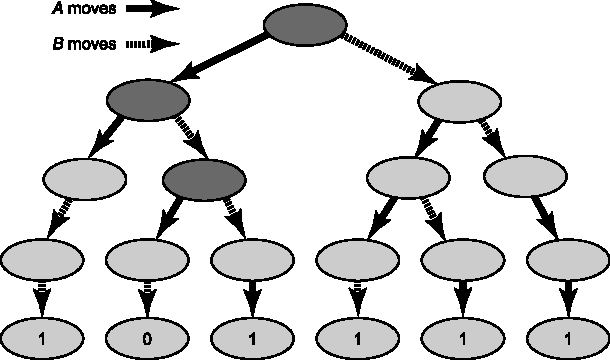
\includegraphics[width=\linewidth,align=t]{ch05 - TAoMP - fig_5.2}
\end{splitquestion}



% 2: Monte Carlo Method for $\pi$
\question
\begin{splitquestion}{0.1}
\Bloom{REMEMBER}
Lorem ipsum dolor sit amet, consectetur adipisicing elit, sed do eiusmod tempor incididunt ut labore et dolore magna aliqua. Ut enim ad minim veniam, quis nostrud exercitation ullamco laboris nisi ut aliquip ex ea commodo consequat \(r = 1\) (see illustrative figure on the right)?
\nextpart
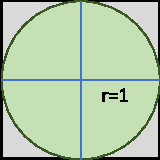
\includegraphics[width=\linewidth,align=t]{P01 Monte Carlo PI Java - fig1}
\end{splitquestion}
\begin{choices}[4]
\choice \(\rho = \pi^2\)
\CHOICE \(\rho = \frac{\pi}{4}\)
\choice \(\rho = \frac{1}{\pi}\)
\choice \(\rho = \frac{4}{\pi}\)
\end{choices}




\end{questions}

%========================================================
% Document ends here
\end{document}


